\section{Theorie}
Ein Hohlleiter ist ein Metallrohr, indem Energie transportiert werden kann.
In diesem Versuch wird ein rechteckiger Hohlleiter verwendet, es gibt aber
auch elliptische oder runde Hohlleiter.

In einem Hohlleiter können
elektromagnetische Schwingungen in verschiedenen Moden weitergeleitet werden.
Jeder Modus besitzt eine Cut-Off-Frequenz, welche durch die Abmessung des
Hohlleiters bestimmt wird. Unter dieser Frequenz kann keine Energie
weitergeleitet werden.
Es wird zwischen zwei Moden unterschieden: der "transversal elektrischen"
(TE-Modus) und der "transversal magnetischen" (TM-Modus) Mode. Hierbei steht das
jeweilige Feld überall senkrecht auf der Ausbreitungsrichtung bzw. der
Hohlleiterachse. Ein Spezialfall ist die Überlagerung beider Moden: Bei dem
TEM-Modus steht sowohl das magnetische als auch das elektrische Feld senkrecht
zur Ausbreitungsrichtung (wie bei einer freien elektromagnetischen Welle oder
einem Koaxialleiter). Die Indizes an dem Modus beschreiben die Anzahl der
Halbwellen des Feldes in die zwei Hauptrichtungen. Als Beispiel ist in Abbildung
\ref{abb:1} der $\text{TE}_{\symup{1,0}}$-Modus in einem rechteckigen Hohlleiter
zu sehen.

\begin{figure}
  \centering
  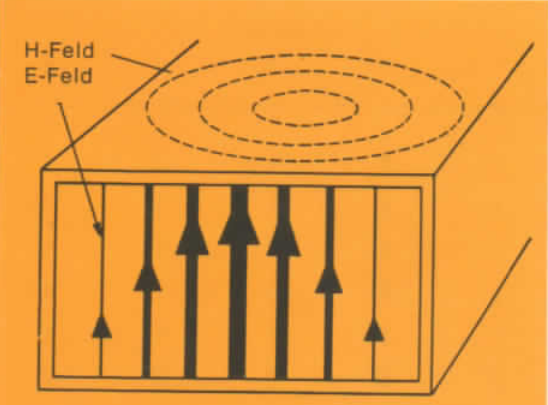
\includegraphics[scale=0.25]{Mode_1_0.png}
  \caption{$\text{TE}_{\symup{1,0}}$-Modus in einem rechteckigen Hohlleiter.
  \cite{Q1}}
  \label{abb:1}
\end{figure}

In Abbildung \ref{abb:2} ist das Blockschaltbild eines Klystron zu sehen.
Ein Klystron ist eine Mikrowellenröhre, bei der aus einem kontinuierlichen
Elektronenstrahl mittels Geschwindigkeitsmodulation Mikrowellenenergie gewonnen
wird. Hierbei werden Elektronen aus der Kathode emittiert und in Richtung der
Gitter beschleunigt.
Aufgrund der Fermi-Dirac-Verteilung besitzen die Elektronen unterschiedliche
Anfangsgeschwindigkeiten, wenn diese aus der Kathode austreten. Der Reflektor
hat gegenüber der Kathode ein negatives Potential, sodass die Elektronen
reflektiert werden. Somit durchlaufen die Elektronen erneut das Resonatorgitter.
Durch die unterschiedlichen Geschwindigkeiten der Elektronen, entstehen bei der
Reflexion Bündel aus Elektronen, da schnelle Elektronen näher zur Kathode
gelangen als langsame Elektronen.
Fängt das Klystron nun an zu schwingen, werden die eintretenden Elektronen, je
nach Ausrichtung des elektrischen Feldes, entweder abgebremst oder beschleunigt.
Bei einer Abbremsung geben die Elektronen einen Teil ihrer Energie an den
Resonator ab, das Klystron schwingt. Die stärkste Schwingung tritt bei einer
Verweilzeit im Resonator von $n+\frac{3}{4}$ der Periodendauer auf
($n \in \mathbb{N}$). Bei einer Beschleunigung nehmen die Elektronen Energie
vom Klystron auf und es entsteht keine Schwingung.

\begin{figure}
  \centering
  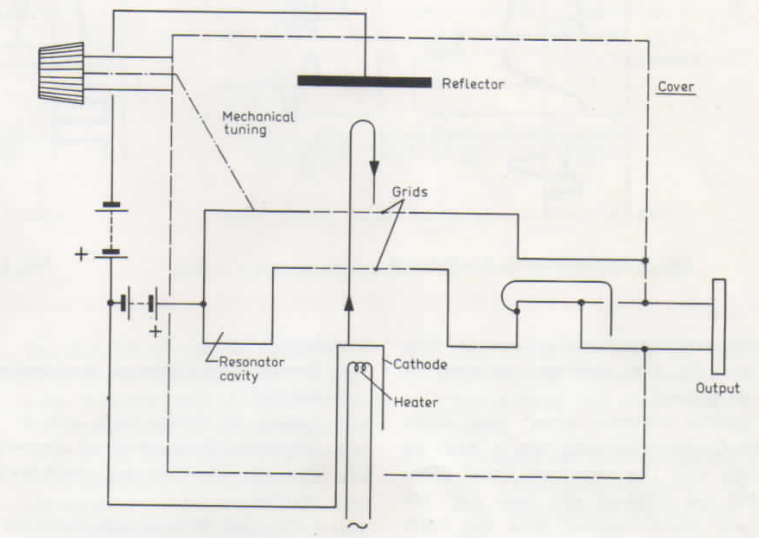
\includegraphics[scale=0.4]{Blockschaltbild.png}
  \caption{Blockschaltbild des Klystrons.\cite{Q1}}
  \label{abb:2}
\end{figure}

In Abbildung \ref{abb:3} sind die Zusammenhänge zwischen Reflektorspannung,
Ausgangsleistung und Schwingungsfrequenz dargestellt. Zu erkennen ist, dass nur
bei bestimmten Reflektorspannungen Schwingen auftreten, da diese von der
Laufzeit der Elektronen abhängt. Diese Schwingen werden auch Moden genannt.
Da die Frequenz direkt von der Abmessung des Resonatorhohlraums abhängt, ist
durch Veränderung des Resonatorvolumens eine \textbf{mechanische Abstimmung} des
Klystrons möglich. Durch Veränderung der Reflektorspannung lässt sich die
Frequenz auch minimal ändern, dies wird \textbf{elektronische Abmessung} genannt.


\begin{figure}
  \centering
  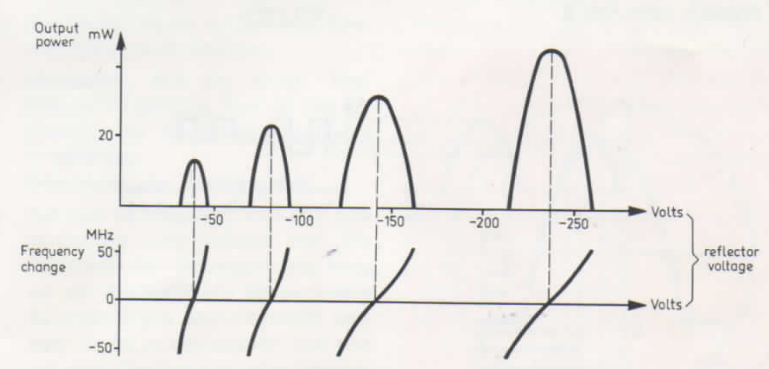
\includegraphics[scale=0.4]{Graph1.png}
  \caption{Zusammenhang zwischen Reflektorspannung, Ausgangsleistung und
  Schwingungsfrequenz. \cite{Q1}}
  \label{abb:3}
\end{figure}

Die Sinusmodulation über die Reflektorspannung ist in Abbildung \ref{abb:4a}
dargestellt.
Falls die Ausgangsleistung über ein SWR-Meter angezeigt werden soll, so muss das
Klystron Amplitudenmoduliert werden. Für eine Rechteckspannung ist dies in
Abbildung \ref{abb:4b} a) dargestellt. In Abbildung \ref{abb:4b} b) ist das
gleiche Ergebnis zu sehen, nur hierbei wurde die Modulationsspannung wie in der
Abbildung zu sehen angelegt. Für die Modulierung ist neben der richtigen
Modulationsspannung auch die richtige Amplitude wichtig.

\begin{figure}
  \centering
  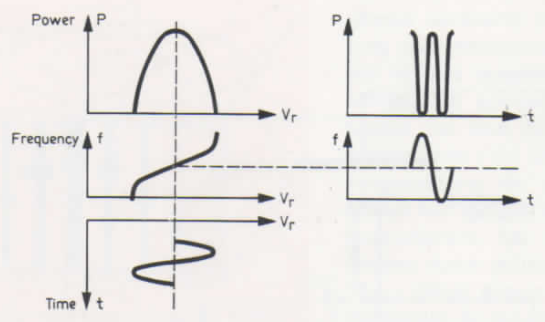
\includegraphics[scale=0.4]{Sinusmodulation.png}
  \caption{Sinusmodulation. \cite{Q1}}
  \label{abb:4a}
\end{figure}
\begin{figure}
  \centering
  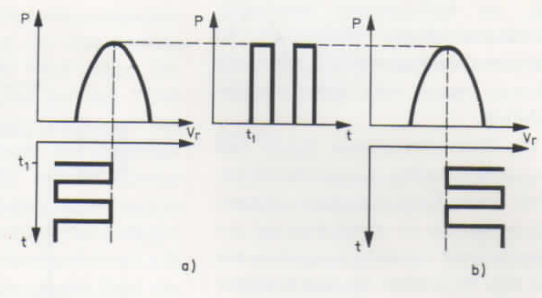
\includegraphics[scale=0.4]{Rechteckmodulation.png}
  \caption{Rechteckmodulation. \cite{Q1}}
  \label{abb:4b}
\end{figure}

\subsection{Frequenz und Wellenlänge}

In einem luftgefüllten Rechteckhohlleiter gilt allgemein für die
$\text{TE}_{\symup{m,n}}$-Mode oder die $\text{TM}_{\symup{m,n}}$-Mode:
\begin{equation}
  \lambda_g =  \frac{\lambda_0}{\sqrt{1-\left(\frac{\lambda_0}{\lambda_c}\right)^2}}
  \label{eq:lambda_g}
\end{equation}
mit
\begin{equation}
  \lambda_c = \frac{2}{\sqrt{\left(\frac{m}{a} \right)^2 + \left(\frac{n}{b} \right)^2}}
  \label{eq:lambda_c}
\end{equation}
($\lambda_0$ Wellenlänge im freien Raum, $\lambda_g$ Wellenlänge im Hohlleiter,
$\lambda_c$ Grenzwellenlänge im Hohlleiter, $a$ Breitseite des Hohlleiters, $b$
Schmalseite des Hohlleiters)

Da ein Hohlleiter meistens in der niedrigsten Mode verwendet wird gilt hier für
die $\text{TE}_{\symup{1,0}}$-Mode oder die $\text{TM}_{\symup{1,0}}$-Mode:
\begin{equation}
  \lambda_c = \frac{2}{\sqrt{\left(\frac{1}{a} \right)^2 + \left(\frac{0}{b} \right)^2}} = 2a
  \label{eq:lambda_c_TE01}
\end{equation}
und damit für die Wellenlänge im Hohlleiter:
\begin{equation}
  \lambda_g =  \frac{1}{\sqrt{1-\left(\frac{\lambda_0}{2a}\right)^2}}
  \label{eq:lambda_g_TE01}
\end{equation}
Mit der Beziehung $f=\frac{c}{\lambda_0}$ folgt für die Frequenz:
\begin{equation}
  f = c \cdot \sqrt{\left(\frac{1}{\lambda_g}\right)^2+\left(\frac{1}{2a}\right)^2}
 \end{equation}
 Die Hohlleiterwellenlänge kann durch den doppelten Abstand zwei
 aufeinanderfolgender Minima (oder Maxima) im Stehwellenfeld direkt gemessen werden.
Bei der Grenzfrequenz ist $\lambda_g$ unendlich groß, das bedeutet, dass sich
das Feld entlang des Hohlleiters nicht ändert. Somit kann auch keine Energie
transportiert werden.

\subsection{Dämpfung}
Die Dämpfung wird gewöhnlich in Dezibel angegeben:
\begin{equation}
  \left(\frac{P_1}{P_2}\right)_{\symup{dB}} = 10 \cdot (\log{P_1}-\log{P_2})
\end{equation}
mit dem Leistungsverhältnis $\frac{P_1}{P_2}$.
In diesem Versuch wird ein Semipräzisionsabschwächer verwendet.

\subsection{Stehwellenmessung}
In dem Hohlleiter überlagern sich die einfallende und die reflektierte Welle.
Diese entsteht durch Unstetigkeiten in der Leitung oder durch eine Lastimpedanz.
Haben beide Wellen die gleiche Phasenlage, entsteht durch die Überlagerung eine
maximale Feldstärke.
Der Spannungs-Reflexionskoeffizient $\rho$ ist definiert als das Verhältnis
zwischen der emittierten und der reflektierten Welle.
Das Spannungs-Schwellen-Verhältnis (SWR) wird durch das Verhältnis der
maximalen und der minimalen Feldstärke der stehenden Welle beschrieben.
Zur Bestimmung der Welligkeiten gibt es mehrere Verfahren:
\begin{itemize}
  \item \textbf{Direkte Messung}: Über eine Sonde (Antenne) kann ein Teil des
  elektrischen Feldes ausgekoppelt werden und auf einem SWR-Meter sichtbar
  gemacht werden. Hierbei darf die Sondentiefe nicht zu groß sein, um das
  elektrische Feld nicht zu sehr zu stören. Die Welligkeit kann direkt an
  dem SWR-Meter abgelesen werden.
  \item \textbf{3dB-Methode}: Hierbei wird der Abstand zwischen zwei Punkten ($d_1-d_2$)
  gemessen, an denen die Detektorspannung das doppelte des Minimums beträgt.
  \begin{equation}
    S= \sqrt{a+\frac{1}{\left(\sin{\frac{\pi(d_1-d_2)}{\lambda_g}}\right)^2}}
    \approx \frac{\lambda_g}{\pi (d_1-d_2)}
  \end{equation}
  Die Näherung in gilt für $S>10$.
  \item \textbf{Abschwächer-Methode}: Das Ausgangssignal des Detektors im Maximum
  wird dem Signal im Minimum mit Hilfe des Abschwächers gleichgemacht. Aus der
  Differenz des Abschwächers lässt sich das SWR berechnen:
  \begin{equation}
    A_2-A_1 = 20 \log{S}
  \end{equation}
\end{itemize}

\section{Durchführung}

\subsection{Untersuchung des Reflexklystrons}

Der Versuch wird wie in Abbildung \ref{abb:Aufbau1} zu sehen aufgebaut.

\FloatBarrier
\begin{figure}
  \centering
  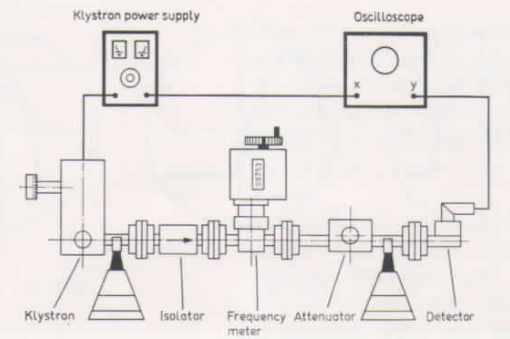
\includegraphics[scale=0.5]{Aufbau1.png}
  \caption{Aufbau zur Untersuchung des Klystrons. \cite{Q1}}
  \label{abb:Aufbau1}
\end{figure}
\FloatBarrier

Das Dämpfungsglied wird auf \SI{40}{\dB}. Die Amplitude der Sinusspannung wird so
eingestellt, dass sich eine horizontale Linie parallel zur Mittellinie ergibt.
Die Reflektorspannung wird auf etwa \SI{200}{\volt} eingestellt, diese wird
so lange variiert, bis die Modenkurve im Mittelpunkt des Oszilloskopes liegt
(siehe Abbildung \ref{abb:Versuch1.1}).
Der Frequenzmesser wird so abgestimmt, dass eine Sattelung an der Spitze der
Modenkurve entsteht. Dabei soll die Frequenz bei etwa \SI{9}{\giga\hertz} liegen.
Weicht die Frequenz zu sehr von dem Wert ab, muss die Amplitude der Sinusspannung
oder der Abstimmknopf des Klystrons variiert werden, sodass
bei einer Frequenz von \SI{9}{\giga\hertz} die gewünschte Sattelung entsteht
(siehe Abbildung \ref{abb:Versuch1.2}).
Die Frequenz und die Resonatorspannung wird abgelesen.
Den Frequenzmesser verstimmen, sodass keine Sattelung mehr vorhanden ist und die
Amplitude ablesen. Die Reflektorspannung so einstellen, dass der Rand der
Modenkurve in der Mitte des Oszilloskops liegt wie in Abbildung
\ref{abb:Versuch1.3} und die Reflektorspannung ablesen. Das gleiche mit der
anderen Seite der Mode durchführen.

\FloatBarrier
\begin{figure}
  \centering
  \begin{subfigure}{0.2\textwidth}
    \raggedleft
    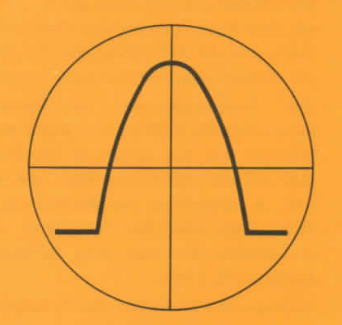
\includegraphics[width=0.93\textwidth]{Versuch1.1.png}
    \caption{}
    \label{abb:Versuch1.1}
  \end{subfigure}
  \begin{subfigure}{0.2\textwidth}
    \centering
    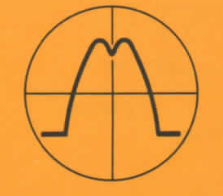
\includegraphics[width=\textwidth]{Versuch1.2.png}
    \caption{mit Sattelung}
    \label{abb:Versuch1.2}
  \end{subfigure}
  \begin{subfigure}{0.2\textwidth}
    \raggedright
    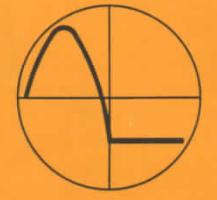
\includegraphics[width=0.955\textwidth]{Versuch1.3.png}
    \caption{Breitenmessung}
    \label{abb:Versuch1.3}
  \end{subfigure}
  \caption{Modenkurven.\cite{Q1}}
\end{figure}
\FloatBarrier

Für die elektronische Abstimmung wird die Reflektorspannung so moduliert, dass
die Sattelung erneut erreicht wird. Die Frequenz und die Reflektorspannung wird
notiert. Die Frequenz wird so variiert, das die Modenkurve auf dem Oszilloskop
der Modenkurve in den Abbildungen \ref{abb:Versuch1.4} und \ref{abb:Versuch1.5}
gleicht. Auch hier wird jeweils die Frequenz und die Reflektorspannung notiert.

\begin{figure}
  \centering
  \begin{subfigure}{0.3\textwidth}
    \raggedleft
    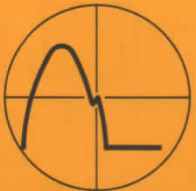
\includegraphics[width=0.58\textwidth]{Versuch1.4.png}
    \caption{}
    \label{abb:Versuch1.4}
  \end{subfigure}
  \begin{subfigure}{0.3\textwidth}
    \raggedright
    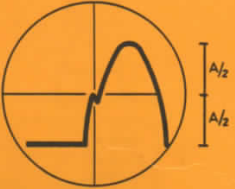
\includegraphics[width=0.7\textwidth]{Versuch1.5.png}
    \caption{}
    \label{abb:Versuch1.5}
  \end{subfigure}
  \caption{Modenkurven elektronische Abstimmung.\cite{Q1}}
\end{figure}

\subsection{Messung von Frequenz, Wellenlänge und Dämpfung}

Der Versuch wird nach Abbildung \ref{abb:Versuch2.Aufbau} umgebaut.

\FloatBarrier
\begin{figure}
   \centering
  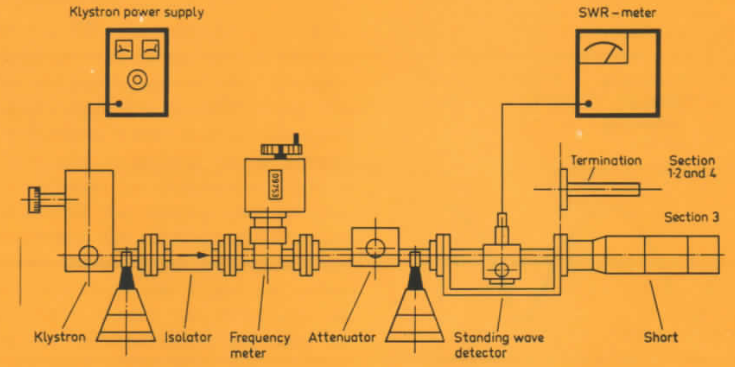
\includegraphics[scale=0.3]{Versuch2.Aufbau.png}
  \caption{Aufbau zur Messung der Frequenz, Wellenlänge und Dämpfung. \cite{Q1}}
  \label{abb:Versuch2.Aufbau}
\end{figure}
\FloatBarrier

Das Dämpfungsglied wird auf \SI{20}{\dB} und die Reflektorspannung auf etwa
\SI{200}{\volt} eingestellt. Am SWR-Meter werden \SI{40}{\dB} und eine Bandbreite von
\SI{100}{\hertz} eingestellt. Mit Hilfe des \SI{1}{\kilo\hertz}-Reglers einen
maximalen Ausschlag erzeugen.

Für die direkte Frequenzmessung den Frequenzmesser modulieren, bis ein Minimum
auf dem SWR-Meter zu erkennen ist. Die Frequenz notieren.

Den festen Abschluss durch den verstellbaren Abschluss ersetzen und den
Frequenzmesser verstimmen. Es werden nun mit Hilfe der Sonde die Punkte
minimalen Ausschlags gesucht und notiert.

Zur Messung der Dämpfung wird erneut der feste Abschluss montiert und der
Frequenzmesser auf \SI{9000}{\kilo\hertz} eingestellt. Die Verstärkung des
SWR-Meters wird so variiert, bis ein Maximum auf dem SWR-Meter zu erkennen ist.
Das Dämpfungsglied wird so eingestellt, sodass die Dämpfung bei \SI{0}{\dB}
liegt. Die Mikrometeranzeige ablesen und notieren. Den Vorgang bis \SI{10}{\dB}
in \SI{2}{\dB}-Schritten wiederholen.

\subsection{Stehwellen-Messungen}

Für den letzten Versuchsteil wird der Versuchsaufbau nach Abbildung
\ref{abb:Versuch3.Aufbau} verändert.

\FloatBarrier
\begin{figure}
  \centering
  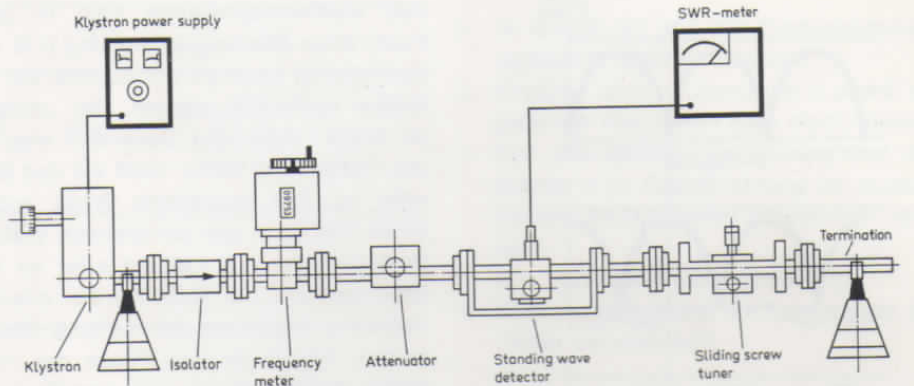
\includegraphics[scale=0.3]{Versuch3.Aufbau.png}
  \caption{Aufbau Stehwellen-Messungen. \cite{Q1}}
  \label{abb:Versuch3.Aufbau}
\end{figure}
\FloatBarrier

Der Abschwächer wird auf \SI{20}{\dB} eingestellt. Am SWR-Meter wird die
Bandbreite auf \SI{20}{\hertz} umgestellt und der \SI{40}{\dB}-Knopf gedrückt.
Die Sonde zur Messung der Feldstärke wird auf Höhe der roten Linie festgeschraubt.
Die Sonde des Gleitschraubentransformators wird ganz herausgedreht.
Das Klystron wird mit \SI{9000}{\kilo\hertz} und einer Rechteckmodulation
(\SI{1000}{\hertz}) zum Schwingen gebracht.

Zur Messung der kleinen und mittleren Welligkeiten die Sondentiefe des
Gleitschraubentransformators auf 3, 5, 7 und 9\,mm einstellen und jeweils ein
Minimum und ein Maximum  durch Verschieben der Messsonde suchen und die Abstände
notieren.

Bei der "\SI{3}{\dB}-Methode" werden nun große Welligkeiten gemessen. Die Sonde
des Gleitschraubentransformators wird auf \SI{9}{\milli\meter} gestellt und es
wird erneut ein Minimum mittels der Messsonde gesucht. Mit Hilfe des Verstärkers
am SWR-Meter wird die Anzeige auf \SI{3}{\dB} verstellt. Die Messsonde wird nun
nach links verschoben, bis die Anzeige des SWR-Meters \SI{0}{\dB} anzeigt und
die Position der Messsonde ablesen. Das gleiche wird erneut durchgeführt, nur dass
die Messsonde nach rechts verschoben wird.

Den Gleitschraubentransformator und den veränderbaren Abschluss durch den
festen Abschluss ersetzen. Mittels der Messsonde den Abstand zwei
aufeinanderfolgender Minima ausmessen.

Zuletzt wird die Abschwächer-Methode durchgeführt:
Erneut den Gleitschraubentransformator und den festen Abschluss in den
Versuchsaufbau einfügen. Die Sondentiefe des Gleitschraubentransformator auf
\SI{9}{\milli\meter} einstellen und die Messsonde in ein Minimum verschieben.
Das Dämpfungsglied auf $A_1=\SI{20}{\dB}$ und die Verstärkung des SWR-Meters
einstellen, sodass der Ausschlag bei \SI{3}{\dB} liegt. Durch Veränderung des
Dämpfungsglieds bei Verschieben der Messleitung wird das relative Maximum
bestimmt.
